\documentclass[11pt]{article}
\usepackage[T1]{fontenc}
\usepackage{lmodern}
\usepackage[margin=1.02in]{geometry}
\usepackage{amsmath,amssymb,amsthm,mathtools}
\usepackage{microtype,booktabs,longtable,array}
\usepackage{enumitem}
\usepackage{listings,xcolor}
\usepackage{tikz}
\usetikzlibrary{arrows.meta,positioning}
\usepackage{fancyhdr}
\usepackage[hidelinks]{hyperref}
\usepackage{bookmark}
\hypersetup{
 pdftitle={Optimal Rank-Two Braid Kernels and Survivor Growth},
 pdfauthor={Research artifact prepared for ProveIt},
 pdfsubject={Certified braid compression and explicit complexity barriers},
 pdfkeywords={unknot recognition, braid groups, certified algorithms, Khovanov homology}
}
\setlength{\headheight}{14pt}
\pagestyle{fancy}
\fancyhf{}
\fancyhead[L]{\small Certified braid compression}
\fancyhead[R]{\small ProveIt research contribution}
\fancyfoot[C]{\thepage}
\setlength{\parskip}{4pt}
\setlength{\parindent}{1.1em}
\setlist{itemsep=3pt,topsep=5pt}
\lstset{basicstyle=\ttfamily\small,breaklines=true,columns=fullflexible,
  keepspaces=true,frame=single,framerule=.3pt,xleftmargin=3pt,xrightmargin=3pt}
\newtheorem{theorem}{Theorem}[section]
\newtheorem{lemma}[theorem]{Lemma}
\newtheorem{proposition}[theorem]{Proposition}
\newtheorem{corollary}[theorem]{Corollary}
\theoremstyle{definition}
\newtheorem{definition}[theorem]{Definition}
\newtheorem{example}[theorem]{Example}
\theoremstyle{remark}
\newtheorem{remark}[theorem]{Remark}
\newcommand{\B}{\mathrm B}
\newcommand{\F}{\mathbb F}
\newcommand{\Z}{\mathbb Z}
\newcommand{\Q}{\mathbb Q}
\newcommand{\Kh}{\widetilde{\mathrm{Kh}}}
\newcommand{\id}{\mathrm{id}}
\newcommand{\supp}{\operatorname{supp}}
\newcommand{\NF}{\operatorname{NF}}
\newcommand{\len}{\operatorname{len}}
\newcommand{\poly}{\operatorname{poly}}
\newcommand{\eps}{\varepsilon}
\newcommand{\tr}{\operatorname{tr}}
\newcommand{\closure}[1]{\widehat{#1}}
\newcommand{\snapshot}{\texttt{0090314cfcc2}}
\title{\textbf{Optimal Rank-Two Braid Kernels\newline and Survivor Growth}\\[6pt]
\large Certified compression for unknot recognition,\newline constructive quasi-polynomial classes, and explicit barriers}
\author{Research artifact prepared for the ProveIt project\\
\small Computer-assisted draft with proofs, independently checked code, and reproducible data}
\date{7 October 2026 \quad\textbar\quad Version 1.0}
\begin{document}
\maketitle
\thispagestyle{empty}
\begin{abstract}
We develop a context-safe preprocessing algorithm for an explicit braid word of
length $n$ on $s$ strands. It computes an optimal collection of disjoint subwords
supported on at most two Artin-generator indices, each replaced by the identity
or one generator. Exact persistent states for $\B_3$ and a weighted prefix
recurrence give deterministic $O(n\log(n+2))$ word-RAM time and $O(n)$ words of
memory, independent of the strand count apart from word size. A separate central
normal form verifies a linear-size rewrite transcript in linear word-RAM time,
even when many shortening passes are composed.

The resulting recognizer has bit complexity
$O(n\log^2(n+s+2))+\poly(k)2^{O(k)}$, where $k$ is the residual crossing count.
In particular, flat rank-two inflations of $O(\log^2 n)$-crossing cores form a
constructively recognized quasi-polynomial class. An explicit arbitrary-strand
family reduces from $8m+s+23$ letters to $s-1$ letters in one pass.

We also prove two limitations. First, any circleless matching-sum complex for
the weaving-braid prefix $(\sigma_1\sigma_2^{-1})^m$ has at least
$\lceil(\lambda^m+\lambda^{-m}-2)/4\rceil$ individual summands when $3\nmid m$,
where $\lambda=(3+\sqrt5)/2$. Thus constant boundary width does not bound explicit
survivor multiplicity, even for prefixes of diagrams whose final closure is the
unknot. Second, an explicit infinite family of four-braid unknots admits no
strictly shortening rank-two substitution, even with arbitrarily long targets.
These are precise barriers to two possible routes to a universal bound, not
complexity lower bounds for unknot recognition itself. The package includes
33 unit tests, 62,352 exhaustive optimization instances, 87,381 algebraic
cross-checks, and paired microbenchmarks. No unrestricted quasi-polynomial
recognizer or full upstream performance improvement is claimed.
\end{abstract}
\vfill
\noindent\textbf{Artifact status.} Mathematical proofs and standard-library Python
implementation are supplied for independent review. The existing repository was
inspected at a pinned commit; its full test suite was not rerun. The opt-in
integration adapter is supplied, not merged. No Lean formalization is claimed.
\clearpage
\tableofcontents
\clearpage

\section{Research question, repository audit, and main conclusions}
\subsection{The concrete optimization problem}
A scanning Khovanov recognizer repeatedly constructs and simplifies a chain
complex. Improvements to arithmetic in one morphism space do not automatically
control the number of objects or differential entries that must survive. Our
starting question is therefore not merely how to multiply a cobordism faster,
but how to avoid constructing a complicated complex for a subword that can
already be replaced by a much smaller braid.

The proposed primitive is deliberately stronger than a local closure test.
Given a contiguous braid subword $u$, a replacement by $v$ is permitted only
when $u=v$ in the braid group, with the same labelled endpoints. Such a
replacement is valid inside \emph{every} surrounding braid context. Merely
knowing that $\closure u$ and $\closure v$ are isotopic is insufficient.

We solve a precise optimization problem for all two-index subwords at once.
A naive approach enumerates quadratically many intervals and solves a group
word problem for each. The central algorithm replaces that enumeration by a
bounded-overlap decomposition and an exact prefix-state dynamic program. The
output is optimal for the stated one-pass rule set, rather than the result of
a greedy search whose choices might exclude better replacements.

\subsection{What was already present}
The inspected ProveIt snapshot is the full commit
\begin{center}
\texttt{0090314cfcc21e1f28ecbc6e8ce4d3f2d99ee743}.
\end{center}
Its \texttt{Topology/UnknotRecognition/fast/fastunknot/braid.py} already
contains a closed-three-braid gateway based on cyclic normal forms in
$C_2*C_3$, an independent integral Burau backend, and a Bennequin obstruction.
The companion \texttt{braid\_reduction.py} performs free/cyclic cancellation
and singleton-endpoint Markov descent. The root README describes structural,
component-sharing, interlacement, and sparse-Alexander stages, and explicitly
does not assert a general quasi-polynomial implementation \cite{repo}.

This contribution does \emph{not} repackage closed-three-braid classification
as a new result. Its new-to-the-inspected-code primitive uses \emph{noncyclic}
states for exact equality of arbitrary local two-index subwords, optimizes all
eligible intervals in one pass, and supplies a separate replay verifier.
The full upstream pipeline was not executed in this environment. Statements
about its source-level gateway are distinguished below from measurements of
our implementation.

Lackenby's July 2026 preprint gives a hierarchy-based incompressibility and
unknot-recognition algorithm. Section 9 bounds iterations by $L(g+1)^L$, but
does not provide sufficiently specified costs for all individual operations;
Section 10 supplies a linear hierarchy-length bound in the initial
$q$-complexity for a refined procedure \cite[\S\S9--10]{lackenby2026}.
Neither that iteration count nor the improvements in this article constitute
an end-to-end universal quasi-polynomial running-time proof.

\subsection{Claims and nonclaims}
The principal positive statements are Theorem~\ref{thm:optimal}, the optimal
rank-two pass; Theorem~\ref{thm:replay}, linear-size replay; and
Theorem~\ref{thm:core}, a constructive quasi-polynomial class. The principal
negative statements are Theorem~\ref{thm:survivors}, exponential matching
multiplicity at constant width, and Theorem~\ref{thm:barrier}, a geodesic
obstruction to every strictly shortening rank-two rule.

The group presentation, the Khovanov unknot-detection theorem, and the weaving
Jones/determinant formula are established background, not priority claims of
this article. The algorithmic synthesis, certificates, explicit comparisons of
positive and negative families, and associated proofs are the contribution
presented here. We have not established priority against every publication on
braid algorithms or weighted word reduction. In particular, whole-braid normal
form algorithms can also recognize some of the artificial identity sleeves
used in our stress tests; the intended advantage here is a small, exactly
optimized, context-safe preprocessing stage with transparent cost accounting.

The supplementary \texttt{openai/math} repository was consulted at the level of
its README and catalogue navigation. Its README distinguishes different
verification stages \cite{openai-math}. No unreviewed theorem from that
collection is used as a premise here.

\section{Input model and exact local braid equality}
\subsection{Explicit words and permitted contexts}
Let
\[
 \B_s=\left\langle \sigma_1,\ldots,\sigma_{s-1}\;\middle|\;
 \begin{array}{ll}
 \sigma_i\sigma_j=\sigma_j\sigma_i&(|i-j|\ge2),\\
 \sigma_i\sigma_{i+1}\sigma_i=\sigma_{i+1}\sigma_i\sigma_{i+1}
 \end{array}\right\rangle .
\]
An input consists of $s\ge1$ and an explicit signed word
$w=g_0\cdots g_{n-1}$, with $g_j\in\{\pm1,\ldots,\pm(s-1)\}$.
We write $\sigma_{g}$ for $\sigma_{|g|}^{\operatorname{sign}(g)}$ and usually
identify a signed word with the corresponding product. Letter positions are
zero-based, and $w[i:j]$ denotes the half-open interval $[i,j)$.

The exponent sum $e(w)=\sum_j\operatorname{sign}(g_j)$ is a homomorphism
$\B_s\to\Z$. In particular, equal words have equal length modulo two.
The support $\supp(w)$ is the set of absolute generator indices occurring in
$w$. A \emph{rank-two word} means a word with $|\supp(w)|\le2$, not a braid
with at most two strands. Adjacent indices act on three strands; distant
indices act on two disjoint pairs.

The optimizer works for links as well as knots. Recognition additionally
requires that the induced permutation be one cycle. A braid whose closure is
a knot must satisfy $s\le n+1$: at least $s-1$ adjacent transpositions are
needed to connect all strand labels. We check this necessary bound before
allocating an $s$-entry permutation array. The bit length of a valid
knot-closure input is $O(n\log(n+s+2))$.

The word-RAM bounds use words of $\Theta(\log(n+s+2))$ bits. Conservative bit
bounds count integer comparisons, arithmetic, and indexing with this size.
No conversion from an arbitrary planar diagram to a braid is hidden in the
model. A separate bounded-cost extraction procedure would be required to
transfer these bounds to unrestricted diagram inputs.

\subsection{Why two indices are special}
One generator gives an infinite cyclic subgroup, and two nonadjacent
generators give $\Z^2$. Their exact states are one or two signed exponent
counts. Two adjacent generators $a=\sigma_i$, $b=\sigma_{i+1}$ generate a copy
of $\B_3$. These subgroup embeddings are faithful: forgetting the stationary
outside strands recovers the three-strand braid, while forgetting to each of
the two moving pairs detects the independent exponents in the distant case.
Thus equality proved in the local group is equality in the ambient braid
context, and conversely.

For the adjacent case put
\[
 x=aba,\qquad y=ab,\qquad z=x^2=y^3.
\]
Eliminating $a,b$ in the Artin relation gives
\begin{equation}\label{eq:presentation}
 \B_3=\langle x,y\mid x^2=y^3\rangle,
 \qquad a=y^{-1}x,\quad b=x^{-1}y^2.
\end{equation}
Indeed, $x^2=(aba)(bab)=(ab)^3=y^3$. Conversely, in the displayed
presentation the definitions $a=y^{-1}x$, $b=x^{-1}y^2$ give $ab=y$ and
$aba=x=bab$, so they recover the Artin relation without an additional
quotient. The element $z$ commutes with both $x$ and $y$. Its exponent sum in Artin
letters is $6$. Quotienting by $z$ gives the free product $C_2*C_3$.

\begin{lemma}[Faithful quotient/exponent pair]\label{lem:faithful}
For $u,v\in\B_3$,
\[
 u=v\quad\Longleftrightarrow\quad
 \bigl(\NF_{C_2*C_3}(u),e(u)\bigr)
 =\bigl(\NF_{C_2*C_3}(v),e(v)\bigr),
\]
where the normal form is reduced, but \emph{not cyclically reduced}.
\end{lemma}
\begin{proof}
The kernel of the quotient map in \eqref{eq:presentation} is the normal
closure of $z$. Since $z$ is central, that kernel is exactly $\langle z\rangle$.
Equal quotient images therefore imply $uv^{-1}=z^q$ for some integer $q$.
Equal exponent sums imply $6q=0$, hence $q=0$. The converse is immediate.
\end{proof}

Reduced quotient words alternate between the order-two token $x$ and a
nonidentity order-three token $y$ or $y^2$. The four letter images are
\begin{equation}\label{eq:images}
 a\mapsto y^2x,\quad a^{-1}\mapsto xy,\quad
 b\mapsto xy^2,\quad b^{-1}\mapsto yx.
\end{equation}
Appending a token either pushes it, cancels an equal-family top token, or
combines two order-three powers modulo three. Every Artin letter uses exactly
two such token updates. A stack consequently computes a reduced word in
linear time, but copying the entire stack after every prefix would be
quadratic. The next section avoids that copying.

\subsection{Two essential soundness guards}
Cyclic reduction is appropriate for some closed-braid questions but loses
local equality information. For example, $a$ and $b$ are conjugate in $\B_3$
and have the same exponent sum, but $a\ne b$. Replacing $a$ by $b$ in the
context $a^{-1}$ changes $aa^{-1}$ to $ba^{-1}$. The former has three
components upon closure; the latter has a three-cycle permutation and hence
one component. This is already a failure at the level of component count.

Likewise, the quotient state alone is not faithful. The full twist
$z=(aba)^2$ has empty quotient normal form but is not the identity, since
$e(z)=6$. Our optimizer stores the exponent sum in every adjacent-group key;
our verifier checks the central lift by a different calculation. Both guards
have explicit regression tests.

\subsection{The independent central normal form}\label{sec:central}
The replay verifier does not import the optimizer's persistent trie. It uses
\[
 z^q f_1\cdots f_r,
\]
where the $f_j$ alternate between $x$ and one of $y,y^2$. Each Artin letter has
a positive-factor expansion with one central correction:
\begin{equation}\label{eq:centralimages}
 a=z^{-1}y^2x,\quad a^{-1}=z^{-1}xy,\quad
 b=z^{-1}xy^2,\quad b^{-1}=z^{-1}yx.
\end{equation}
The reductions are $xx\to z$ and
$y^i y^j\to z^{\lfloor(i+j)/3\rfloor}y^{(i+j)\bmod3}$, omitting the
identity factor. Updating the central integer and an alternating stack takes
constant word-RAM work per factor.

For completeness, this representation is unique. Its alternating word is
fixed by the reduced normal form in $C_2*C_3$; once that word is fixed, the
central power is fixed by the exponent sum. A representation of the identity
therefore has empty alternating part and central exponent zero. To check
$u=v$ for a one-letter or empty target, the verifier reduces $uv^{-1}$ by
\eqref{eq:centralimages}. The search and verification implementations share
input validation but not their group-state algorithms.

\section{Bounded-overlap corridors and persistent prefix states}
\subsection{All maximal two-index intervals in linear size}
\begin{definition}
A \emph{corridor} is a maximal nonempty interval of the input whose letters
use at most two absolute generator indices. If the entire word uses just one
index, it is the unique corridor. For a nonhomogeneous word we take the
maximal two-index intervals, which also contain every one-index subinterval.
\end{definition}

\begin{lemma}[Corridor overlap bound]\label{lem:corridors}
All corridors can be computed in $O(n)$ word-RAM time. Every rank-two
subinterval lies in a corridor. At any letter position at most two corridors
are active, and the sum of their lengths is at most $2n$.
\end{lemma}
\begin{proof}
Compress maximal runs with the same absolute index, retaining each run's
start and end positions. Consecutive runs have distinct labels. Label the
edge between two consecutive runs by the unordered pair of their labels.
A maximal string of equal edge labels specifies exactly a maximal interval
using that pair of indices. When edge labels change, consecutive corridors
share precisely the intervening run. Distinct nonconsecutive corridors are
disjoint. Thus each run, and each original letter, belongs to at most two
corridors. Any interval using at most two labels extends to one of these
maximal intervals. The run and edge scans are linear.
\end{proof}

\begin{figure}[ht]
\centering
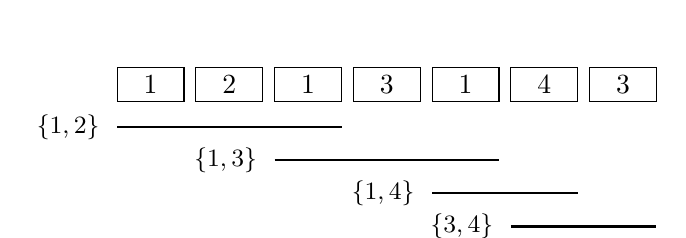
\begin{tikzpicture}[x=1.0cm,y=.65cm]
\foreach \x/\label in {0/1,1/2,2/1,3/3,4/1,5/4,6/3}{
 \draw (\x,0) rectangle ++(.85,.65);
 \node at (\x+.425,.325) {$\label$};
}
\draw[thick] (0,-.5)--(2.85,-.5);
\node[anchor=east] at (-.1,-.5) {\small $\{1,2\}$};
\draw[thick] (2,-1.15)--(4.85,-1.15);
\node[anchor=east] at (1.9,-1.15) {\small $\{1,3\}$};
\draw[thick] (4,-1.8)--(5.85,-1.8);
\node[anchor=east] at (3.9,-1.8) {\small $\{1,4\}$};
\draw[thick] (5,-2.45)--(6.85,-2.45);
\node[anchor=east] at (4.9,-2.45) {\small $\{3,4\}$};
\end{tikzpicture}
\caption{Corridors after run compression. Each box denotes a run, not
necessarily a single letter. Neighboring corridors overlap in one run, so
all local group scans together read at most $2n$ input letters.}
\label{fig:corridors}
\end{figure}

\subsection{Exact persistence without fingerprints}
Represent each reduced $C_2*C_3$ word by a node in a rooted trie. A node has a
parent pointer, its final token, and three child pointers, one for each
possible token. The root is the empty word. A push uses the corresponding
child, creating it if necessary; a cancellation returns the parent; a
nonzero order-three combination uses the appropriate child of the parent.
Every node is consequently a canonical exact word identifier.

This is not a probabilistic hash of a potentially long group word. Node
identity is justified by the trie construction itself. Child lookup uses a
fixed array of size three, so it has deterministic constant cost. The
optimizer may share this trie between all adjacent corridors: their local
indices are consistently relabelled $a,b$, and their prefix tables remain
separate.

At a position $j$ inside a corridor starting at $\ell$, let $p_j$ denote the
local product $w[\ell:j]$. Its adjacent-group key is a pair consisting of the
trie node and the exponent sum. A distant-group key is its two exponent
counts. The singleton case uses one count and a zero second coordinate.

For a target $v$ of length zero or one, the algorithm needs the state of
$p_jv^{-1}$. In the adjacent case it performs at most one additional
persistent Artin update; no input prefix is copied or rescanned. In the
commuting case it subtracts one exponent. The identity target needs no
extra group update.

\begin{proposition}[State construction bounds]\label{prop:states}
For a radius-one pass, there are at most $2n$ input group advances, at most
$10n$ target-state queries, at most $20n$ quotient-token updates, and at most
$20n+1$ trie nodes. All exact state identifiers and scores fit in
$O(\log(n+s+2))$ bits.
\end{proposition}
\begin{proof}
There are at most five targets in any corridor: the identity and four signed
generators. Each corridor letter causes one input advance and at most four
query advances, each consisting of two token updates. Apply
Lemma~\ref{lem:corridors}. A token update creates at most one node. Signed
prefix exponents, positions, and savings have magnitude $O(n)$.
\end{proof}

\section{An optimal shortening pass}
\subsection{The exact admissible rule set}
Fix $r\in\{0,1\}$. A legal interval replacement is
\[
 w[i:j]\longmapsto v,
\]
where $|\supp(w[i:j])|\le2$, $v$ is the empty word when $r=0$, and when $r=1$
it may also be one signed generator from that support. It must represent the
same local braid, and $j-i>|v|$. A one-pass plan consists of disjoint legal
intervals in the \emph{current input word}. Its savings are
$\sum(j-i-|v|)$. The output retains every uncovered letter unchanged.

The restriction to targets in the interval's support is explicit. For the
radius-one problem it does not silently ignore a single-generator equality:
in the one- and two-index parabolic subgroups the relevant generator cannot
be replaced by an outside adjacent transposition. We nonetheless build this
restriction directly into both the definition and the verifier rather than
relying on an implicit ambient test.

\subsection{Weighted prefix recurrence}
Let $F[j]$ be the maximum savings achievable on $w[0:j]$, with $F[0]=0$.
For each active corridor, keep a table $H$ indexed by exact local group
states. After processing start positions $i$ in that corridor, the table
stores
\begin{equation}\label{eq:table}
 H(q)=\max_{i:\ p_i=q}\bigl(F[i]-i\bigr),
\end{equation}
with an attaining position for backtracking. The maximum over an empty set
is absent. Ties use the earlier position.

The elementary equivalence
\begin{equation}\label{eq:prefixidentity}
 w[i:j]=v\quad\Longleftrightarrow\quad p_i=p_jv^{-1}
\end{equation}
turns all candidate starts into one lookup per target. We obtain
\begin{equation}\label{eq:dp}
 F[j]=\max\left\{F[j-1],\quad
   j-|v|+H(p_jv^{-1}):
   \text{active corridors and their permitted targets }v\right\}.
\end{equation}
A corridor beginning at $j$ is initialized with its identity state and
value $F[j]-j$. At each endpoint, all candidate queries are made before
inserting that endpoint into each table. This ensures that only previously
available start positions are used.

A candidate need not separately be discarded for zero savings. If it
strictly improves on $F[j-1]$, then its interval has positive savings,
since $F[j-1]\ge F[i]$. Equal candidates do not replace the inherited plan.
Parity of exponent sum then shows that every selected replacement saves
at least two letters.

\begin{theorem}[Optimal rank-two pass]\label{thm:optimal}
For an explicit $n$-letter braid word, the algorithm above computes an
optimal one-pass plan for $r=0$ or $r=1$. With deterministic AVL prefix tables
it uses
\[
 O(n\log(n+2))\text{ word-RAM time},\qquad O(n)\text{ words of memory}.
\]
A conservative bit-time bound is $O(n\log^2(n+s+2))$, with
$O(n\log(n+s+2))$ bits of memory. The optional ordinary hash-table backend
has expected linear dictionary work under its usual hashing assumptions;
that is not the deterministic guarantee.
\end{theorem}
\begin{proof}
Induct on the processed endpoint $j$. In an optimal plan for the prefix,
either no selected interval ends at $j$, so the plan is available in
$F[j-1]$, or its last selected interval is $[i,j)$ with target $v$. The part
before it has savings at most $F[i]$, and its total is therefore at most
$F[i]+j-i-|v|$. Conversely, an optimal prefix plan attaining $F[i]$ can be
followed by that interval, since the two parts are disjoint.

Every permitted interval lies in a corridor by Lemma~\ref{lem:corridors}.
Equation~\eqref{eq:prefixidentity} is exact by the local group normal forms.
For a fixed corridor and target, maximizing over valid starts is exactly
\eqref{eq:table}. Consequently \eqref{eq:dp} includes all possible last
intervals and returns the true optimum. Storing the chosen start and target
or an inherited-prefix pointer reconstructs an optimal plan.

Proposition~\ref{prop:states} bounds the group updates and queries linearly.
Each AVL access has $O(\log(n+2))$ comparisons. At most one table entry is
inserted per active corridor endpoint, so all table nodes, trie nodes,
scores, backpointers, and corridors occupy $O(n)$ words. The reconstructed
output is at most $n$ letters long. Charging $O(\log(n+s+2))$ bit operations
to a word-sized comparison, arithmetic operation, or index manipulation
gives the stated conservative bit bound.
\end{proof}

\subsection{Pseudocode and an important nongreedy feature}
\begin{lstlisting}[caption={Optimal disjoint shortening; exact group states are implicit.}]
F[0] := 0
for j = 1,...,n:
    initialize each corridor beginning at j-1 using F[j-1]
    F[j] := F[j-1]; choice[j] := KEEP
    for each active corridor C:
        advance its prefix state by w[j-1]
        for v in {empty, permitted signed one-letter targets}:
            old := H_C[state(prefix_C * inverse(v))]
            if old exists and j - length(v) + old.score > F[j]:
                F[j] := j - length(v) + old.score
                choice[j] := (old.position, v)
    for each active corridor C:
        update H_C[state(prefix_C)] with (F[j]-j, j)
    retire corridors ending at j
backtrack choice[] and emit the resulting disjoint replacements
\end{lstlisting}

An individual corridor is not simplified independently and then spliced
back. Such an approach can conflict on overlapping runs. The common array
$F$ carries the global prefix optimum into every corridor's table, and
backtracking selects disjoint intervals across corridor boundaries. This is
the reason the overlap lemma yields an exact global one-pass result rather
than a collection of locally optimal but incompatible choices.

\subsection{Repeated passes and their actual guarantee}
After one pass, new neighboring letters may expose a rank-two interval that
was not contiguous in the original word. The function \texttt{compress}
therefore allows repeated optimal passes. Each nontrivial pass saves at
least two letters, so at most $\lfloor n/2\rfloor$ such passes occur. A final
no-op pass witnesses saturation under the chosen radius.

\begin{corollary}\label{cor:repeat}
Repeated rank-two shortening terminates in deterministic
$O(n^2\log(n+2))$ word-RAM time and $O(n^2\log^2(n+s+2))$ conservative bit
time, with $O(n)$ words of live algorithmic storage plus its transcript.
The final word has no eligible strict shortening at the selected radius.
\end{corollary}
\begin{proof}
Sum the one-pass bound over at most $\lfloor n/2\rfloor+1$ passes, each of
length at most $n$. Store only the current pass's state structures, the
shrinking word, persistent letter IDs, and the accumulated linear transcript
proved below. A no-op optimal pass implies that no positive-savings eligible
interval exists.
\end{proof}

Saturation does not mean global geodesicity or unknot recognition. The bound
also does not prove that repeated passes choose a globally best sequence of
future rewrites. Theorem~\ref{thm:barrier} supplies an infinite family on which
even perfect local geodesic shortening cannot start.

\section{Linear-size certificates and independent replay}
\subsection{Stable nodes rather than repeated word snapshots}
A certificate that stores the entire intermediate word after every pass can
use quadratic space even when all valid deletions are simple. Instead assign
original letters stable IDs $0,\ldots,n-1$. During replay they form a doubly
linked list. A replacement records only
\[
 (\texttt{first},\texttt{last},\texttt{target}),
\]
where the first and last IDs are live endpoints of a contiguous interval,
and the target is zero for the identity or the signed inserted generator.
An inserted target receives the next fresh ID. The verifier follows the
live successor pointers between the supplied endpoints, checks the exact
local equality, and splices the target into the list.

The certificate also records the strand count, original length, an input
SHA-256 digest, the selected radius, and a claimed final word. The final word
is recomputed from replay rather than trusted. The digest is a provenance
check, not the basis for mathematical equality: every step is checked against
the actual input letters. An empty or prematurely stopped transcript is
legal and proves only its listed equalities, not saturation or optimality.

\begin{theorem}[Linear accounting for all replayed passes]\label{thm:replay}
Any valid transcript of strict rank-two replacements by targets of length at
most one has at most $n/2$ steps and introduces at most $n/2$ new letter nodes.
Across the entire replay, at most $3n/2$ nodes are removed. Consequently the
transcript has $O(n\log(n+s+2))$ bits and can be verified in $O(n)$ word-RAM
time and $O(n\log(n+s+2))$ conservative bit time.
\end{theorem}
\begin{proof}
An equality preserves exponent sum modulo two, so strict shortening by a
zero- or one-letter target removes at least two more letters than it
introduces. There can be at most $n/2$ steps, and each introduces at most one
node. A node can be removed at most once. If $I$ nodes are introduced and $R$
are removed, then
\[
 I\le n/2,\qquad R\le n+I\le3n/2.
\]
Following live intervals therefore visits at most $3n/2$ removed nodes in
total. Group verification of an interval uses its length plus at most one
target letter, by Section~\ref{sec:central} or the commuting exponent check.
All local checks together are linear. Pointer updates are constant per
replacement. Initial input validation and final traversal are also linear.
IDs are bounded by $3n/2$, targets by $s-1$, and central counters by the
interval lengths, giving the bit and certificate-size bounds.
\end{proof}

The complexity claim concerns well-formed bounded-size certificates. For an
adversarially oversized serialized document, its parsing and integer input
size must also be charged. The implementation rejects more than $n/2$ steps,
invalid or dead IDs, reversed endpoints, forbidden targets, false equalities,
and final-word mismatches. A failed interval traversal adds at most one
current-word scan before rejection; it does not invalidate the amortization
of previously accepted steps.

\subsection{The trust boundary}
The search routine is not part of the equality verifier's trusted logic.
An erroneous optimizer can lose performance or return a rejected certificate;
it cannot justify a false equality merely by reporting a favorable score.
The verifier itself remains ordinary Python and mathematical proof, not a
proof-assistant-verified kernel. Its independence is strengthened by checking
against the faithful Artin action in small cases, a matrix/exponent encoding
in $\B_3$, and Khovanov ranks on small diagrams. Finite testing cannot replace
the proof or eliminate every implementation defect.

We intentionally do not certify that the supplied plan is optimal. Checking
optimality can rerun the deterministic dynamic program. The compact replay
format certifies the property needed to preserve the recognizer's verdict:
\emph{the reduced word is the same braid as the original word}.

\section{From compressed crossing count to quasi-polynomial classes}
\subsection{A complete exponential fallback with explicit accounting}
The established unknot-detection theorem states that a knot has reduced
Khovanov homology of rational rank one exactly when it is the unknot
\cite{kronheimer-mrowka}. The same rank-one criterion works over $\F_2$:
the universal coefficient theorem bounds rational rank above by the
$\F_2$ dimension, and the unknot has dimension one over either field.
The rational rank cannot be zero, for example by the normalized Jones Euler
characteristic. We use this only for one-component closures.

\begin{lemma}[Elementary cube bound]\label{lem:cube}
For a $k$-crossing knot diagram, the reduced Khovanov cube over $\F_2$ can be
constructed and its total rank computed in $\poly(k)2^{O(k)}$ bit time.
One conservative explicit bound is $\poly(k)2^{6k}$.
\end{lemma}
\begin{proof}
There are $2^k$ resolutions. Starting from one immersed knot component,
changing the local pairing at each of the $k$ crossings can increase the
number of components by at most one, so every full resolution has at most
$k+1$ circles. Mark one circle. The reduced state space then has dimension
$2^{c-1}\le2^k$, since the marked circle is fixed to the $x$ label in
$A=\F_2[x]/(x^2)$. The entire reduced chain space has dimension
$D\le2^{2k}$.

For each cube edge, the Frobenius multiplication or comultiplication has
constant local branching, and all resolution connectivity can be generated
with polynomial overhead per state and edge. A conservative dense
$\F_2$ elimination bound is $O(D^3)$ bit operations; constructing the
matrices costs at most a further polynomial factor in $k$ times an
exponential already absorbed in the displayed bound. Thus
$\poly(k)2^{6k}$ is sufficient. For a differential $d$ on the total chain
space, $d^2=0$ gives $\dim H=D-2\operatorname{rank}(d)$.
\end{proof}

The included \texttt{cube.py} implements this elementary expanded cube for
validation and as a reference backend. It is not proposed as a replacement
for the repository's much more sophisticated scanner. It defaults to a
12-crossing cap and a 100,000-vector cap; exceeding either yields
\texttt{INCONCLUSIVE}, not a mathematical verdict. Setting both caps to
\texttt{None} selects the uncapped exponential backend used in the theorem.

\subsection{A structural input class rather than a guessed width bound}
\begin{definition}[Flat rank-two inflation]
A word $w$ is a flat rank-two inflation of a word $c$ if it can be obtained by
replacing selected letters of $c$ by nonempty rank-two words equal to those
letters and inserting rank-two identity words between letters. The inserted
or substituted blocks are pairwise disjoint in $w$. Their locations and the
core $c$ are not supplied to the algorithm. Let $\kappa_1(w)$ be the minimum
output length over the radius-one one-pass rule set.
\end{definition}

Leaving a letter unchanged is permitted. Identity blocks may be omitted when
empty. Substitutions of length one can also be left unchanged, so requiring
strict shortening for selected rules does not affect the following bound.
The adjective ``flat'' excludes nested substitutions whose outer support
becomes rank two only after inner replacements have been removed.

\begin{theorem}[Constructive core-compression bound]\label{thm:core}
Let $w$ be an $n$-letter braid whose closure is a knot. One deterministic
radius-one pass computes a same-braid word with exactly $\kappa_1(w)$ letters.
Following it by the uncapped reduced-cube recognizer gives bit complexity
\begin{equation}\label{eq:hybrid}
 O(n\log^2(n+s+2))+
 \poly(\kappa_1(w))\,2^{O(\kappa_1(w))}.
\end{equation}
If $w$ is a flat rank-two inflation of a $k$-letter core, then
$\kappa_1(w)\le k$. Hence every such family with
$k=O(\log^2(n+2))$ is recognized in $\exp(O(\log^2(n+2)))$ bit time.
\end{theorem}
\begin{proof}
The exact optimum is Theorem~\ref{thm:optimal}; its replay certificate is
Theorem~\ref{thm:replay}. Same-braid equality preserves the closure, so the
output is a knot. If it has $\kappa_1$ letters, its strand count is at most
$\kappa_1+1$, eliminating any hidden strand factor in the cube construction.
Lemma~\ref{lem:cube} and the rank-one criterion prove \eqref{eq:hybrid}.

The disjoint inflated blocks themselves specify a legal plan with output
length at most $k$. Optimality therefore produces no longer an output even
though that decomposition was not given. Substituting
$k\le C\log^2(n+2)$ into the exponential term gives the claimed
quasi-polynomial time. The preprocessing and replay are smaller than that
bound.
\end{proof}

This is an unconditional theorem \emph{on the explicitly defined input
class}. It is not the unproved assertion that all unknot diagrams lie in that
class. Membership in the bounded-$\kappa_1$ class is itself decidable by the
same optimal pass. An adversarially expanded input may have a small core;
an already compact but difficult diagram may not. The result supplies a
useful compositional parameter, not a universal complexity classification.

\subsection{A composition principle for better backends}
Nothing in the shortening proof is specific to Khovanov homology. Suppose a
correct backend decides the closure of a $k$-letter residual braid in time
$T(k)$. Preprocessing and verification give
\[
 O(n\log^2(n+s+2))+T(\kappa_1(w))
\]
bit time, provided conversion to that backend is charged in $T$. This is the
recommended integration viewpoint: shrink the true diagram, preserve a
replayable map from the original input, and retain every already proved
filter or backend. Do not replace a rigorous backend by a heuristic
interpretation of the shortening score.

\section{An arbitrary-strand family solved in one pass}
\subsection{Central-commutator sleeves}
For adjacent generators $a,b$ and $m\ge1$ define
\[
 \beta_m(a,b)=(ab^{-1})^m,\qquad z(a,b)=(aba)^2,
\]
\begin{equation}\label{eq:sleeve}
 E_m(a,b)=\beta_m(a,b)\,z(a,b)\,\beta_m(a,b)^{-1}\,z(a,b)^{-1}.
\end{equation}
The element $z$ is central in the local $\B_3$, so $E_m=1$. Its literal
length is $4m+12$. It need not contain an adjacent inverse cancellation:
its two long sides encode a nontrivial equality through the central element.

For $s\ge4$ let
\[
 \delta_s=\sigma_1\sigma_2\cdots\sigma_{s-1},
\]
\begin{equation}\label{eq:family}
 w_{s,m}=E_m(\sigma_1,\sigma_2)\,
 E_m(\sigma_{s-2},\sigma_{s-1})\,\delta_s.
\end{equation}
This has length $8m+s+23$ and represents $\delta_s$.

\begin{theorem}[One-pass optimal compression of the sleeve family]\label{thm:sleeves}
For every $s\ge4$ and $m\ge1$, either radius-zero or radius-one optimal
shortening reduces $w_{s,m}$ to a word of length exactly $s-1$. The residual
word is positive and contains every generator index exactly once. Its
closure is the unknot. Thus this arbitrary-strand family is recognized in
polynomial time, and in near-linear preprocessing time apart from any
chosen generic downstream implementation of the final certificate.
\end{theorem}
\begin{proof}
The two displayed sleeve intervals are disjoint rank-two identity words.
Deleting them is a legal radius-zero plan with $s-1$ residual letters. On
the other hand, $e(w_{s,m})=s-1$, so no equal word can have fewer than $s-1$
letters. The optimum is therefore exactly $s-1$ at either radius.

Every residual letter must be positive to attain that exponent bound. Its
permutation is that of $\delta_s$, a single $s$-cycle. If some index $i$ were
absent, its adjacent transpositions would preserve the two sets
$\{1,\ldots,i\}$ and $\{i+1,\ldots,s\}$, contrary to being an $s$-cycle.
There are $s-1$ letters and $s-1$ required indices, so each occurs once.

A positive word containing each index once has unknot closure. Indeed, its
rightmost endpoint generator $\sigma_{s-1}$ occurs exactly once; cyclically
rotate the word to place it at an end and destabilize. The remaining word
again contains each of the $s-2$ remaining indices exactly once. Induction
reaches the one-strand unknot. The same argument works with all signs
negative, which justifies the conservative signed-Coxeter shortcut in the
reference recognizer.
\end{proof}

The actual reference shortcut checks length, common sign, and distinct
indices in $O(n+s)$ word work. Although arbitrary sign choices with each
index once admit a similar endpoint argument, the supplied shortcut only
accepts the uniform-sign condition it explicitly checks.

\subsection{What the inspected raw-word gateway does on this family}
The words in \eqref{eq:family} are freely and cyclically reduced. The first
endpoint index appears $2m+9$ times, and the last appears $2m+5$ times.
Neither is a singleton. Their exponent sum $s-1$ meets, rather than
violates, the gateway's Bennequin threshold. Since $s>3$, the closed-three-
braid branch is not directly applicable.

Consequently the inspected \texttt{braid\_certificate} code takes its
inconclusive path on these inputs before our shortening step. Afterwards,
its singleton descent can act on the $s-1$-letter positive residual word.
This is a source-level branch analysis, not a measured claim that the full
upstream pipeline was slow. A diagram-level reduction, another filter, or
another normal form might already handle these examples efficiently. The
supplied optional integration smoke test checks this narrower gateway
prediction when executed in a real checkout.

\subsection{Why the stress family is still informative}
The number of alternating blocks in $\beta_m$ grows with $m$; the family is
not confined to a fixed number of long twists. More importantly, its prefix
has large unavoidable homological complexity in an explicit matching basis,
as proved next, even though the complete input has a short algebraic
certificate. This distinguishes ``fast local arithmetic'' from ``avoiding
an unnecessarily expanded intermediate object.'' It does not distinguish
our method from every known whole-braid normal form algorithm.

\section{Exponential survivor multiplicity at constant boundary width}
\subsection{The precise representation under discussion}
Bar-Natan's tangle formalism and scanning algorithm provide the relevant
categorical setting \cite{bar-natan-tangles,bar-natan-fast}. Work over $\F_2$.
After delooping, a formal chain object is a direct sum of grading-shifted
circleless crossingless matchings with the fixed tangle boundary. Define
$R(C)$ to be the total number of \emph{individual} such summands over all
homological degrees, including repeated copies and grading shifts.

This is the quantity counted by an explicit object-basis implementation.
It is not the number of distinct matching \emph{types}, and it is not the
size of an arbitrary succinct circuit that could represent a complex.
A compressed multiplicity count, tensor expression, or decision-only
invariant need not pay $R(C)$ in storage. The lower bound below is scoped to
this explicit matching-sum model.

\subsection{A determinant growing exponentially}
Let
\[
 \beta_m=(\sigma_1\sigma_2^{-1})^m\in\B_3,
 \qquad W_m=\closure{\beta_m}.
\]
The permutation of $\sigma_1\sigma_2^{-1}$ is a three-cycle. Thus $W_m$ is a
knot when $3\nmid m$. In the reduced Burau representation at $t=-1$,
\[
 A=\begin{pmatrix}1&1\\0&1\end{pmatrix},\qquad
 B=\begin{pmatrix}1&0\\-1&1\end{pmatrix},\qquad
 M=AB^{-1}=\begin{pmatrix}2&1\\1&1\end{pmatrix}.
\]
The established closed-three-braid Jones trace formula, specialized to the
exponent-zero braid $\beta_m$, gives
\begin{equation}\label{eq:det}
 d_m=|V_{W_m}(-1)|=\tr(M^m)-2
     =\lambda^m+\lambda^{-m}-2,
 \qquad \lambda=\frac{3+\sqrt5}{2}.
\end{equation}
This is also the known formula $d_m=L_{2m}-2$ for the weaving determinant
\cite[\S2, Corollary 3.5]{weaving}. The calculation needs only the matrix
shown above: its characteristic polynomial is $X^2-3X+1$, which yields
\[
 T_0=2,\quad T_1=3,\quad T_{m+1}=3T_m-T_{m-1},\qquad d_m=T_m-2.
\]
We use this recurrence for exact integer checks, without floating-point
approximation of $\lambda^m$.

\begin{lemma}[Euler-characteristic rank bound]\label{lem:euler}
For a knot $K$, $\dim_{\F_2}\Kh(K;\F_2)\ge |V_K(-1)|$.
\end{lemma}
\begin{proof}
The normalized Jones polynomial is the graded Euler characteristic of the
reduced Khovanov complex, hence of its homology, after the conventional
change of variable and grading normalization. At $t=-1$ all grading
monomials have absolute value one. The triangle inequality bounds the
absolute value of that signed graded sum by the sum of all graded
homology dimensions. The argument works over $\F_2$ because Euler
characteristic is an equality of integer dimensions, not a reduction of
polynomial coefficients modulo two.
\end{proof}

\subsection{A closure functional bounds every explicit complex}
\begin{theorem}[Constant-width survivor lower bound]\label{thm:survivors}
Fix $s\ge3$ and $m\ge1$ with $3\nmid m$. Let $C$ be any finite circleless
matching-sum chain complex over $\F_2$, homotopy equivalent in the tangle
category to $\beta_m$ on the first three strands together with $s-3$
vertical strands. Then
\begin{equation}\label{eq:survivorbound}
 R(C)\ \ge\ \left\lceil\frac{d_m}{4}\right\rceil
 =\left\lceil\frac{\lambda^m+\lambda^{-m}-2}{4}\right\rceil.
\end{equation}
The estimate is independent of the cancellation order and of the number
$s$ of added trivial strands.
\end{theorem}
\begin{proof}
Apply the standard braid closure, with a marked point on the $W_m$
component, and then the reduced $\F_2$ Khovanov functor. Homotopy equivalence
is preserved. The closed tangle is the split union of $W_m$ with $s-3$
unknotted circles. Each unmarked split circle tensors the reduced complex
with the two-dimensional Frobenius vector space $A$. Since the ground ring
is a field, the resulting total homology dimension is
\[
 2^{s-3}\dim\Kh(W_m;\F_2)\ \ge\ 2^{s-3}d_m.
\]

A circleless matching on the $2s$ endpoints, after composition with the
closure matching, becomes a disjoint union of at most $s$ circles. To see
this, overlay the two perfect matchings: every resulting alternating cycle
uses at least two endpoints, and there are $2s$ endpoints. With one marked
circle, its reduced vector space has dimension $2^{c-1}\le2^{s-1}$.
Consequently the total vector-space dimension obtained by closing $C$ is
at most $2^{s-1}R(C)$. Homology dimension is at most chain dimension, so
\[
 2^{s-3}d_m\le2^{s-1}R(C).
\]
Cancel the common factor and round up.
\end{proof}

For example, the exact lower bounds for $m=16$ and $m=32$ are respectively
$1{,}217{,}712$ and $5{,}931{,}287{,}624{,}352$ summands. These are theorem-
derived counts, not measurements of an attempted allocation of such a
complex. The input prefixes have only 32 and 64 crossings.

\subsection{The final knot can nevertheless be trivial}
\begin{corollary}\label{cor:easyfinal}
For $s=4$, the unknots $w_{4,m}$ from \eqref{eq:family} have a natural
left-to-right braid-prefix scan with constant boundary size whose
intermediate explicit matching-sum representation requires at least
$\lceil d_m/4\rceil$ summands when $3\nmid m$. The complete input is
compressed to three letters by one optimal rank-two pass.
\end{corollary}
\begin{proof}
The initial $2m$ letters are $\beta_m$ on the first three strands with a
fourth vertical strand. Apply Theorem~\ref{thm:survivors} at that prefix.
The complete input is covered by Theorem~\ref{thm:sleeves}.
\end{proof}

This corollary assumes a scan that actually materializes a homotopy-equivalent
complex at that prefix. It does not force another scan order, a look-ahead
algorithm, an early decision filter, or a succinct symbolic representation
to do so. Nor does it prove exponential running time of the supplied
repository's entire recognizer. What it refutes is the general implication
\[
 \text{constant boundary width}\quad\Longrightarrow\quad
 \text{polynomially many explicit matching summands}.
\]
Thus a width-only argument cannot close the complexity analysis of an
explicit scanner. Bounds on a local nilpotent radical or on one cobordism
algebra must be supplemented by a bound on the actual multiplicity or by a
representation that does not enumerate it.

\section{An infinite obstruction to all strict rank-two shortening}
\subsection{A higher-rank identity with locally geodesic pieces}
Write $a=\sigma_1$, $b=\sigma_2$, $c=\sigma_3$ in $\B_4$. Define
\[
 U=abcaba,\qquad V=cbacbc,\qquad r=UV^{-1}.
\]
The two positive words are equal. Here is a complete derivation using only
one Artin relation or distant commutation on each line:
\begin{align*}
 abcaba&=abacba\\
       &=babcba\\
       &=bacbca\\
       &=bcabca\\
       &=bcabac\\
       &=bcbabc\\
       &=cbcabc\\
       &=cbacbc.
\end{align*}
Thus $r=1$. This is a half-twist coherence identity, not a claim that the
local rank-two group relations fail to generate the braid group. They do
generate it; the crucial restriction below is \emph{strict shortening at
every chosen substitution}.

For $h\ge1$ define
\begin{equation}\label{eq:barrierfamily}
 q_h=r^h\,abc.
\end{equation}
The word has length $12h+3$ and represents $abc=\delta_4$, so its closure is
the unknot.

\begin{theorem}[Geodesic rank-two barrier]\label{thm:barrier}
Every contiguous rank-two subword of $q_h$ is geodesic in its local
one- or two-index group with respect to its signed Artin generators.
Consequently $q_h$ admits no strictly shortening rank-two replacement,
regardless of the allowed target length. Radius-zero and radius-one
shortening, even iterated to saturation, leave it unchanged.
\end{theorem}
\begin{proof}
Within a positive block $U$, all letters have exponent $+1$; within a
negative block $V^{-1}$, all have exponent $-1$; the final $abc$ block is
positive. A uniform-sign word of length $t$ has exponent sum of absolute
value $t$, so no equal word can have fewer than $t$ letters. This proves
geodesicity for every rank-two interval contained in a single sign block.

At a positive-to-negative join, the neighboring letters are $a,c^{-1}$.
The letter just before them, when present, is $b$, and the letter just
after them is $b^{-1}$. Thus any interval crossing that join and supported
on at most two indices is contained in the two-letter word $ac^{-1}$.
At a negative-to-positive join, including the join with the final $abc$,
the corresponding word is $c^{-1}a$, again flanked by index $b$ on both
sides. No two-index interval can span more than one sign boundary.

Since $a$ and $c$ commute and generate $\Z^2$, both mixed two-letter words
have exponent vector $(1,-1)$, whose $\ell^1$ norm is two. They too are
geodesic. Their one-letter subwords are trivially geodesic. These cases
exhaust all rank-two subintervals, proving the assertion.
\end{proof}

\subsection{What must change to escape the obstruction}
Allowing longer \emph{strictly shorter} targets in the same rank-two group
cannot help on this family. A successful extension must use at least one
of the following mechanisms: length-preserving rank-two relations before
shortening, higher-rank equality tests, a different decomposition into local
pieces, or operations that preserve the closed knot rather than the braid
itself, with their own appropriate certificates.

The eight displayed equal-length moves already reveal how to solve this
particular family: rewrite $U$ to $V$, cancel $VV^{-1}$, and repeat. This is
an explicit escape route, not a universal bound on how much such coherent
rewriting is needed. A generic higher-rank normal form can likewise
recognize the identity interval. The practical and asymptotic issue is how
to search these possibilities without introducing an uncontrolled state
space or expensive intermediate representations.

This negative result improves the research specification: a proof that
all unknots reach short cores by strict rank-two shortening is false,
not merely unproved. The broad quasi-polynomial objective must be stated
for a stronger move system or a different algorithm.

\section{Implementation, validation, and measured results}
\subsection{Package structure and executable contracts}
The package is standard-library Python with a \texttt{src} layout.
The production preprocessing path comprises \texttt{kernel.py},
\texttt{search\_group.py}, and \texttt{orderedmap.py}. The independent
certificate path is \texttt{verify.py}. The CLI compresses an input and
verifies the resulting certificate before writing it.

The small-case independent oracles in \texttt{oracles.py} include exhaustive
interval optimization, the faithful Artin action on a free group, and the
$2\times2$ Burau specialization together with exponent sum. The expanded
Artin action can grow exponentially and has a resource guard; it is never
used in the preprocessing complexity bound. The reference cube is likewise
an explicit exponential validation backend.

The public preprocessing call is
\begin{lstlisting}[language=Python]
from ranktwo import compress, verify
result = compress(strands, word, radius=1,
                  max_passes=1, dictionary="avl")
reduced_word, replay = verify(strands, word, result["certificate"])
\end{lstlisting}
Setting \texttt{max\_passes=None} saturates under the selected rules.
Setting \texttt{dictionary="hash"} changes the dictionary implementation,
not the exact equality relation. Deterministic asymptotic claims refer to
\texttt{"avl"}. Budget callbacks are cooperative and exceptions propagate;
they are not hard operating-system time or memory limits.

\subsection{Completed validation}
The recorded environment was CPython 3.13.5 on x86-64 Linux with glibc 2.41.
The 33 unit tests passed. Three additional reproducible sweeps completed
without mismatches:
\begin{center}
\begin{tabular}{p{.54\linewidth}r}
\toprule
Check & Cases\\
\midrule
All $\B_3$ words of length at most 8: persistent quotient/exponent,
central normal form, and matrix/exponent cross-checks & 87,381\\[4pt]
All $\B_3$ words of length at most 7 and all $\B_4$ words of length at most 5,
at both radii, compared with exhaustive interval optimization & 62,352\\[4pt]
Seeded random same-braid comparisons using the expanded Artin action & 1,000\\[4pt]
Seeded random small-diagram Khovanov comparisons before and after reduction & 100\\
\bottomrule
\end{tabular}
\end{center}
Both dictionary backends were run on each exhaustive optimization instance,
for 124,704 optimized dictionary runs. The 100 homology comparisons checked
$d^2=0$ on both cubes, for 200 checked complexes. The random seeds, run
counts, environment, and elapsed times are in the accompanying JSON files.
The algebra sweep found 2,589 distinct group keys; its purpose was agreement
of encodings, not a proof inferred from that finite count.

Regression tests include the full-twist central guard, conjugacy-versus-
equality failure, distant generators, all sign choices of input letters,
empty inputs, malformed data, budget exceptions, multi-pass fresh-node
replay, dead IDs, false targets, altered provenance, altered final words,
AVL balancing, the sleeve family, and the rank-two geodesic barrier.
The test suite also checks known small reduced Khovanov dimensions, including
1 for the unknot, 3 for the trefoil, 5 for the figure-eight knot, and 45
for $W(3,4)$, with the cube differential squared explicitly.

The adapter's three tests inject a fake gateway and check its call and
resource-handling contract. They are \emph{not} tests of the real upstream
implementation. No upstream test total is included in our 33-test count.

\subsection{Paired comparison with interval enumeration}
The following medians use three runs on the same seeded random $\B_3$ word
at each length, with the order of the optimized and brute-force method
randomized inside each pair. Import/setup time is excluded. Every optimum
was checked for agreement.
\begin{center}
\begin{tabular}{rrrrr}
\toprule
Input letters & Output letters & AVL (ms) & Enumeration (ms) & Ratio\\
\midrule
16 & 8  & 0.198 & 2.379 & 12.0\\
32 & 20 & 0.340 & 15.948 & 47.0\\
64 & 12 & 0.606 & 126.119 & 208.0\\
128& 32 & 1.593 & 1006.575 & 631.7\\
\bottomrule
\end{tabular}
\end{center}
These ratios compare our optimized primitive with our deliberately slow,
independent interval oracle. They are not speedups over
\texttt{fastunknot}, not end-to-end recognition measurements, and not evidence
of an asymptotic exponent beyond the proven algorithm analysis.

\subsection{Scaling and an intentionally unsuccessful family}
For the four-strand sleeves, one pass plus separate replay gave:
\begin{center}
\begin{tabular}{rrrrrr}
\toprule
$m$ & Input & Output & AVL (s) & Hash (s) & Replay (s)\\
\midrule
16   & 155   & 3 & 0.007013 & 0.000891 & 0.000185\\
64   & 539   & 3 & 0.019297 & 0.009651 & 0.000519\\
256  & 2075  & 3 & 0.039764 & 0.012942 & 0.002241\\
1024 & 8219  & 3 & 0.157361 & 0.082743 & 0.009492\\
4096 & 32795 & 3 & 0.758853 & 0.229557 & 0.040261\\
\bottomrule
\end{tabular}
\end{center}
Each transcript had two replacements. At 32,795 letters the pass made
32,798 corridor advances and 163,990 state queries; the verifier removed
32,792 original nodes and introduced none. These exact counters are more
portable than elapsed times. The deterministic bound does not require the
hash timings to be favorable.

On the negative family $q_h$, the output length equals the input length, as
proved rather than merely observed:
\begin{center}
\begin{tabular}{rrrr}
\toprule
$h$ & Input = output & AVL (s) & Replay (s)\\
\midrule
8    & 99    & 0.001454 & 0.000052\\
32   & 387   & 0.005504 & 0.000170\\
128  & 1539  & 0.023437 & 0.000666\\
512  & 6147  & 0.098295 & 0.002979\\
2048 & 24579 & 0.450543 & 0.011254\\
\bottomrule
\end{tabular}
\end{center}
These no-op runs are an important guard against reporting only favorable
examples. Their transcripts contain zero replacements; replay still checks
input provenance and the final word. At the largest size the trie has only
24 nodes, yet the optimizer correctly refuses to infer a global identity
from many small recurrent local states.

All timing tables report completed runs. Raw samples, not just medians,
are retained in \texttt{results/benchmarks.json}. The small timing samples
are descriptive; no confidence interval, hardware-independent speed claim,
or distributional knot-complexity conclusion is asserted.

\section{Integration and the route beyond rank two}
\subsection{An opt-in integration order}
The adapter is a separate file rather than a silent modification of the
repository. It first preserves an already decisive raw-braid gateway
result. If that gateway is inconclusive, it applies one rank-two pass,
verifies the transcript, and retries the gateway on the reduced input.
If still inconclusive, it returns that reduced word for the existing
conversion and exact backend. It does not guess the signature of the
repository's planar-diagram constructor or replace its final detector.

A production integration should retain the original word and its transcript
in any returned witness. A result about a reduced diagram must not be
attached to the original input without its replayable reduction. Resource
exceptions should pass into the pipeline's established inconclusive/error
handler. They must never become mathematical verdicts. The initial default
should be one deterministic pass with an explicit time/memory budget;
repeated passes can be a separately measured option.

The supplied \texttt{integration/upstream\_check.py} is intended to run with
the inspected \texttt{fast} directory on \texttt{PYTHONPATH}. It tests the
source-level prediction for 16 sleeve instances. It was not run in the
artifact-building environment, so no compatibility success is reported.
The full production test suite, non-braid inputs, thread races, and the Rust
port remain integration work.

\subsection{A general prefix-state transfer theorem}
The rank-two construction suggests a broader, precise algorithmic interface.
It is useful to separate the dynamic program from the cost of its exact
group representation.

\begin{proposition}[Finite-target prefix transfer]\label{prop:general}
Let $G$ be a finitely generated group with a fixed set $\mathcal V$ of target
words. Suppose exact canonical prefix states can be constructed for the
input and for all $p_jv^{-1}$, $v\in\mathcal V$. Let $U$ bound the work to
construct each such query state, $C$ the cost of comparing two canonical
states, and $S$ the total state storage required. Then the optimal
collection of disjoint replacements of arbitrary subintervals by equal
members of $\mathcal V$ can be found in
\[
 O\bigl(n|\mathcal V|(U+C\log(n+2))\bigr)
\]
time and $O(S+n)$ additional state/score slots, using an ordered dictionary.
Only positive-savings replacements are selected.
\end{proposition}
\begin{proof}
Use a single table for all prefix states of the entire input and repeat
\eqref{eq:table}--\eqref{eq:dp}. The last-interval induction in
Theorem~\ref{thm:optimal} does not require a rank restriction. Charge one
query-state construction and ordered-dictionary lookup per target per
endpoint. The table contains at most $n+1$ prefix entries. The separate
$S$ term includes all canonical state representations and their sharing;
it must not be dropped merely because state identifiers are small.
\end{proof}

Taking all empty and one-letter targets in $\B_s$ would remove the
rank-two locality restriction and would recognize the identity interval
$r^h$ in Section 8. This proposition is not an implementation or a new
cost bound for a higher-rank canonical form. It identifies the exact
primitives to benchmark and bound. In particular, a faithful action stored
as fully expanded free-group words is not automatically a polynomial
implementation: its storage can grow exponentially. Canonical-state
construction, comparison, and persistence must all be costed.

\subsection{What a universal quasi-polynomial theorem would need}
There are at least two distinct programs. A \emph{compression program}
would produce a small residual core, or a recursively decomposed collection
of small certified pieces, in quasi-polynomial time. It must escape the
strict-shortening obstruction and control the size of all intermediate
witnesses. A \emph{hierarchy program} would implement topological cutting and
simplification with bounded-size encoded structures and an end-to-end
operation count. The unresolved operation costs in the published hierarchy
analysis cannot be filled by a statement about the number of high-level
steps alone.

A \emph{succinct homological program} is a third possibility. It would store
complexes or their decision-relevant information without enumerating the
matching summands prohibited by Theorem~\ref{thm:survivors}. It must bound
both representation size and exact operations on that representation.
A small local algebra, a small boundary, or a small number of matching types
is not itself that bound.

The present work supplies an inexpensive and auditable interface between
these programs: exact context-safe compression before expensive topology or
homology. It also supplies two adversarial families that a claimed universal
analysis must explicitly handle.

\section{Further research questions and proposed investigations}
The following questions are intended as testable research tasks, not as
unproved steps silently used above.

\subsection{Higher-rank persistence and coherent rewriting}
\paragraph{1. Canonical prefix states beyond two indices.}
Can a persistent higher-rank braid normal form implement
Proposition~\ref{prop:general} with a useful deterministic bit bound and
small constants? A complete answer must include canonical comparison,
right-multiplication queries, state sharing, and a verifier. The first
benchmark should contain both sleeve and half-twist-barrier families.

\paragraph{2. Short-target radius as a parameter.}
For fixed rank two and radius $r>1$, enumerate target words of length at
most $r$, deduplicate equal group elements, and retain the shortest
representative of each. The same recurrence has a finite target factor,
roughly $4^{O(r)}$, and query construction proportional to $r$. What exact
state and certificate bounds are best? This may enlarge practical cores,
but Theorem~\ref{thm:barrier} proves that increasing $r$ alone cannot solve
all inputs under strict rank-two shortening.

\paragraph{3. Bounded neutral-move budgets.}
Allow a controlled number of length-preserving Artin or commutation moves
before a shortening pass. Can a quasi-polynomial search space be proved for
some nontrivial class, using a potential that charges neutral moves rather
than ignoring them? The eight-step identity $U=V$ is a mandatory initial
regression, but a universal conjecture must also face much more complicated
coherence relations.

\paragraph{4. Event-driven saturation.}
The repeated-pass analysis is quadratic. Can newly exposed corridor
boundaries be updated locally without repeatedly scanning unaffected
segments? The challenge is that prefix optimality scores may change far
from a deletion, even though the word edit is local. Prove an amortized
bound or construct an adversarial family forcing global recomputation.

\subsection{Compression parameters and structural knot classes}
\paragraph{5. Nested inflation depth.}
Define depth-$d$ rank-two inflations where a block becomes rank two only
after its children are simplified. Does an algorithm recover a bounded-
depth decomposition without receiving it as a certificate? An existence
proof must distinguish arbitrary optimal-pass tie choices from a supplied
nested decomposition, since one optimal pass may cross the intended
block boundaries.

\paragraph{6. Observable versus existential core size.}
How does $\kappa_1(w)$ compare with geodesic braid length, reduced diagram
crossing count, or other structural parameters? The barrier family proves
that equality of these notions is false. Quantitative inequalities under
specific geometric hypotheses could turn the present conditional-on-core
bound into a broader structural theorem.

\paragraph{7. Braid patches in general diagrams.}
Develop a deterministic procedure to locate and certify maximal braid-like
patches in a planar diagram, with endpoint order and local orientation
retained. Prove the extraction cost, bound overlap, and ensure that no
expensive global braiding conversion is hidden. Only then can the
rank-two preprocessing theorem be stated directly for unrestricted diagram
encodings with an honest input-size bound.

\paragraph{8. Compression followed by Markov moves.}
Study the interaction between context-safe braid equalities and
closure-preserving destabilization. A useful certificate should keep these
two types of steps distinct. Are there families where alternating the two
reduces a parameter geometrically, rather than merely decreasing crossing
count by two?

\subsection{Avoiding explicit survivor multiplicity}
\paragraph{9. Symbolic tensor and multiplicity representations.}
Can the complexes of weaving prefixes be represented with polynomial-size
exact circuits supporting closure and the rank-one decision, despite the
exponential explicit-summand lower bound? A claimed representation must
also support differential composition and cancellation without an implicit
expansion of its repeated terms.

\paragraph{10. Closure-functional lower bounds for richer models.}
The proof of Theorem~\ref{thm:survivors} uses one closure and one rank
functional. Can a family of closures bound tensor rank, decision-diagram
width, or another succinct representation invariant? Such a theorem could
separate promising compression schemes from encodings that only rename
the same exponential basis.

\paragraph{11. Scan orders with look-ahead certificates.}
The natural sleeve scan is expensive in the explicit model, but early
recognition of its central identity avoids it. Can an order-selection
algorithm use locally certified equalities to guarantee a small maximum
intermediate object on a broad class? Both the cost of finding the order
and the full intermediate representation must be included.

\subsection{Topological hierarchies, formal verification, and deployment}
\paragraph{12. Encoded hierarchy operations.}
For the hierarchy route, specify one nontrivial cutting or weak-reduction
primitive with an explicit input/output format, coordinate bit bounds,
provenance, and measured implementation. A verified cost for such a
primitive would be more decisive than another abstract recurrence with
uncosted steps.

\paragraph{13. Formalize the small trusted core.}
A manageable proof-assistant target is the quotient/exponent injectivity
lemma, persistent-trie invariant, weighted-prefix recurrence, and stable-ID
replay theorem. The Khovanov unknot detector can initially remain an
external theorem in the integration contract. Clearly identify any axioms
or trusted foreign code rather than labelling the entire recognizer
formally verified.

\paragraph{14. Production ablation and Rust port.}
Measure the adapter with the actual upstream raw gateway, then with the
full recognizer on existing examples and adversarial words. Report
preprocessing overhead when no shortening is possible, final verdicts,
backend crossings, peak memory, timeouts, and paired timings. A Rust port
should reproduce certificates and exact optima against the Python oracle
before being judged on performance.

\section{Conclusion}
The deliverable is a proved, implemented optimization primitive rather than
an assertion that all difficult topology has become easy. It replaces
quadratic interval enumeration by exact persistent group states and an
optimal weighted prefix scan. It makes arbitrary-strand local equalities
usable without confusing braid equality with closure equivalence. It also
keeps the trusted replay work linear across repeated passes.

The constructive quasi-polynomial theorem is precise: flat rank-two
inflations of $O(\log^2 n)$-crossing cores are recognized within the desired
asymptotic scale, and the decomposition need not be supplied. The sleeve
family is handled even with arbitrarily many strands by a further elementary
certificate. At the same time, exponentially large explicit matching
multiplicity at constant width and an infinite strict-shortening barrier
rule out two overly optimistic universal arguments.

The next substantial advance should therefore address higher-rank or
length-preserving coherence, a provably succinct decision representation,
or fully costed topological hierarchy operations. The code, transcripts,
positive families, negative families, and exact counters supplied here are
intended to make those future claims sharply testable.

\clearpage
\appendix
\section{Reproduction and artifact inventory}
From the package root, using Python 3.10 or newer:
\begin{lstlisting}[language=bash]
export PYTHONPATH="$PWD/src${PYTHONPATH:+:$PYTHONPATH}"
python -m unittest discover -s tests -v
python experiments/validate.py groups
python experiments/validate.py optimality
python experiments/validate.py independent
python experiments/benchmark.py
python -m ranktwo compress examples/sleeved_unknot_4_16.json \
    --passes 1 --output results/example_compressed.json
python -m ranktwo verify examples/sleeved_unknot_4_16.json \
    results/example_compressed.json
cd paper && sh build.sh
\end{lstlisting}
The package includes \texttt{README.md}, \texttt{CLAIMS.md},
\texttt{INTEGRATION.md}, source modules, unit tests, deterministic generators,
raw benchmark/validation results, worked JSON certificates, the TeX source,
this PDF, a provenance manifest, and SHA-256 checksums. The reproduction
scripts operate locally; they do not require network access. LaTeX rebuilding
requires the packages named in the preamble.

The default CLI performs compression and replay, not unrestricted unknot
recognition. The guarded reference hybrid is available as a Python function.
A capped computation can return \texttt{INCONCLUSIVE}. For complete decision,
retain the production backend or deliberately use the uncapped reference
cube, accepting its exponential resource use.

\section{A short worked certificate}
For $s=4,m=1$, the input $w_{4,1}$ has 35 letters. Its first sleeve occupies
original IDs $0$ through $15$, its second IDs $16$ through $31$, and the
last three letters are $1,2,3$. A radius-zero certificate can therefore
contain the two entries
\begin{lstlisting}
{"first": 0,  "last": 15, "target": 0}
{"first": 16, "last": 31, "target": 0}
\end{lstlisting}
with output word \texttt{[1,2,3]}. Both equalities are checked locally in
$\B_3$ by the central normal form. Neither step invokes the global unknot
detector. The final positive three-letter braid has unknot closure by
endpoint destabilization. The larger worked examples use the same
certificate format; the transcript need not enumerate the potentially long
sequence of elementary Artin moves hidden in one exact local equality.

\clearpage
\section{Status ledger}
\begin{longtable}{p{.27\linewidth}p{.64\linewidth}}
\toprule
Item & Status and scope\\
\midrule
\endhead
Rank-two equality & Proved using the central quotient and exponent sum;
independently implemented central-carry verifier.\\[4pt]
One-pass optimum & Proved for disjoint rank-two substitutions to zero or one
letter; exhaustively checked on the reported finite ranges.\\[4pt]
Repeated saturation & Proved termination and quadratic upper bound; not a
global minimum-length or Markov-equivalence algorithm.\\[4pt]
Quasi-polynomial class & Proved for flat rank-two inflations of
$O(\log^2 n)$ cores; no universal small-core theorem.\\[4pt]
Explicit survivor bound & Proved in the circleless matching-sum model; not
a lower bound for all representations, scan orders, or recognizers.\\[4pt]
Strict-shortening barrier & Explicit infinite family; applies even to
arbitrary target lengths in rank-two local groups.\\[4pt]
Reference cube & Implemented and small-case checked; exponential, guarded
by default; not a practical substitute for the production scanner.\\[4pt]
Upstream integration & Adapter and smoke test supplied; full upstream suite
and smoke test not executed; no repository writes performed.\\[4pt]
Measured speedups & Against the independent brute interval oracle only;
not against the full upstream recognizer.\\[4pt]
Formal verification & Not performed; no Lean certificate or machine-checked
proof-assistant theorem claimed.\\
\bottomrule
\end{longtable}

\clearpage
\begin{thebibliography}{9}
\bibitem{repo}
V. Reshetnikov, \emph{ProveIt: Topology/UnknotRecognition}, repository snapshot
\texttt{0090314cfcc21e1f28ecbc6e8ce4d3f2d99ee743}, inspected 7 October 2026.
Root README; \texttt{fast/fastunknot/braid.py};
\texttt{fast/fastunknot/braid\_reduction.py}.
\url{https://github.com/VladimirReshetnikov/ProveIt/tree/0090314cfcc21e1f28ecbc6e8ce4d3f2d99ee743/Topology/UnknotRecognition}.

\bibitem{lackenby2026}
M. Lackenby, \emph{Incompressible surfaces, hierarchies and unknot recognition},
preprint, arXiv:2607.23350v1, 25 July 2026.
\url{https://arxiv.org/abs/2607.23350}.

\bibitem{bar-natan-tangles}
D. Bar-Natan, \emph{Khovanov's homology for tangles and cobordisms},
Geometry \& Topology \textbf{9} (2005), 1443--1499.
arXiv:math/0410495.
\url{https://arxiv.org/abs/math/0410495}.

\bibitem{bar-natan-fast}
D. Bar-Natan, \emph{Fast Khovanov homology computations},
Journal of Knot Theory and Its Ramifications \textbf{16} (2007), 243--255.
arXiv:math/0606318. DOI:10.1142/S0218216507005294.
\url{https://arxiv.org/abs/math/0606318}.

\bibitem{kronheimer-mrowka}
P. B. Kronheimer and T. S. Mrowka,
\emph{Khovanov homology is an unknot-detector},
Publications math\'ematiques de l'IH\'ES \textbf{113} (2011), 97--208.
arXiv:1005.4346.
\url{https://arxiv.org/abs/1005.4346}.

\bibitem{weaving}
M. E. AlSukaiti and N. Chbili,
\emph{Alexander and Jones polynomials of weaving 3-braid links and Whitney
rank polynomials of Lucas lattice}, Heliyon \textbf{10} (2024), e28945.
DOI:10.1016/j.heliyon.2024.e28945.
\url{https://pmc.ncbi.nlm.nih.gov/articles/PMC11004560/}.

\bibitem{openai-math}
OpenAI, \emph{math}, repository README and catalogue navigation,
consulted 7 October 2026. Supplementary resource only; no manuscript theorem
from this collection is assumed in the present proofs.
\url{https://github.com/openai/math}.
\end{thebibliography}
\end{document}
